\documentclass[10pt,twocolumn,letterpaper]{article}

%%%%%%%%% PAPER TYPE  - PLEASE UPDATE FOR FINAL VERSION
\usepackage{cvpr}              % To produce the CAMERA-READY version
% \usepackage[review]{cvpr}      % To produce the REVIEW version
% \usepackage[pagenumbers]{cvpr} % To force page numbers, e.g. for an arXiv version

% Import additional packages in the preamble file, before hyperref
\usepackage[dvipsnames]{xcolor}
\newcommand{\red}[1]{{\color{red}#1}}
\newcommand{\todo}[1]{{\color{red}#1}}
\newcommand{\TODO}[1]{\textbf{\color{red}[TODO:#1]}}

% It is strongly recommended to use hyperref, especially for the review version.
% hyperref with option pagebackref eases the reviewers' job.
% Please disable hyperref *only* if you encounter grave issues, 
% e.g. with the file validation for the camera-ready version.
%
% If you comment hyperref and then uncomment it, you should delete *.aux before re-running LaTeX.
% (Or just hit 'q' on the first LaTeX run, let it finish, and you should be clear).
\definecolor{cvprblue}{rgb}{0.21,0.49,0.74}
\usepackage[pagebackref,breaklinks,colorlinks,citecolor=cvprblue]{hyperref}


%%%%%%%%% PAPER ID  - PLEASE UPDATE
\def\paperID{*****} % *** Enter the Paper ID here
\def\confName{CVPR}
\def\confYear{2024}

%%%%%%%%% TITLE - PLEASE UPDATE
\title{\ Tsception model for emotion recognition with LSTM\ }

% \author{
%     Kshitiz Kumar\\
%     \texttt{ai22mtech02002@iith.ac.in} \and
%     Tanay Yadav\\
%     \texttt{ai20btech11026@iith.ac.in} \and
%     Tanmay Goyal\\
%     \texttt{ai20btech11021@iith.ac.in} \and
%     Tanmay Shah\\
%     \texttt{ee20btech11061@iith.ac.in}
% }

%%%%%%%% AUTHORS - PLEASE UPDATE
\author{Shreyas Wankhede\\
{\tt\small ai21btech11028@iith.ac.in}
% For a paper whose authors are all at the same institution,
% omit the following lines up until the closing ``}''.
% Additional authors and addresses can be added with ``\and'',
% just like the second author.
% To save space, use either the email address or home page, not both
\and
Omkaraditya Pujari\\
{\tt\small ai20btech11017@iith.ac.in}
}


\begin{document}
\maketitle
\begin{abstract}
    In our study, we have proposed a model called Tsception which is used for emotion recognition. The data consists of EEG signals captured from an experimental set up. The proposed model of Tsception has a CNN architecture with several convolutional blocks. It consists of Temporal and spatial convolutional layers which are respectively used to capture temporal and spatial dependencies.The dynamic temporal layer uses varying sized kernels corresponding to different sampling rates to capture the finer spectra ot temporal patterns. The spatial assymmetric layer learns discriminative patterns between left and right hemispheres. The fusion layer fuses outputs from both convolutional layers and gives a higher level representation of the data. The concatenated output is passed to fully connected layer for training. The study evaluates emotion recognition across two dimensions arousal and valence. The data were collected from 32 subjects to evaluate the model performance. The proposed model is seen to outperform various state of the art methods like SVM, EEGNet, LSTM etc.
\end{abstract}   

\section{Introduction}
Emotions are essential aspects of human life, influencing our daily choices, understanding of the world, social interactions, and cognitive abilities. Consequently, emotion recognition is crucial in therapeutic approaches such as Cognitive Behavioral Therapy (CBT), Emotion Regulation Therapy (ERT), and Emotion-Focused Therapy (EFT). It also plays a vital role in assessing medical interventions for mental health conditions such as Generalized Anxiety Disorder (GAD) and Depression. Hence, there has been growing interest among researchers in leveraging Artificial Intelligence to detect and understand human emotions, especially for applications in CBT and EFT.

Electroencephalography (EEG) is a sophisticated and non-invasive neuroimaging technique that measures and records the electrical activity of the brain. By placing multiple electrodes on the scalp, EEG captures and amplifies the electrical signals produced by the brain's neurons, providing invaluable insights into its function and activity. One of the significant advantages of EEG is its high temporal resolution, allowing researchers and clinicians to observe and analyze rapid changes in brain states at a sub-second level. This temporal precision is particularly beneficial in studying various cognitive processes, emotional responses, and neurological disorders.

In recent years, EEG technology has seen remarkable advancements, especially with the integration of machine learning and signal processing techniques. These technological innovations have enabled the development of sophisticated Brain-Computer Interface (BCI) systems that can interpret and translate EEG signals into actionable insights. BCI systems equipped with EEG-based emotion detection algorithms can identify and classify human emotions, offering new avenues for understanding emotional states and enhancing human-computer interaction. Moreover, EEG-based BCI systems have found applications beyond academic research and clinical settings. They are increasingly being used in various industries, including healthcare, gaming, and assistive technology. In healthcare, EEG helps in diagnosing and monitoring neurological conditions such as epilepsy, sleep disorders, and cognitive impairments. In gaming and virtual reality, EEG-based BCI systems offer immersive and interactive experiences by adapting gameplay in real-time based on the player's cognitive and emotional states. Additionally, in assistive technology, EEG allows individuals with severe motor impairments to communicate and interact with their environment using brain signals, improving their quality of life. Numerous researchers such as Zheng et al., Li et al. and others have come up with various ways for using EEG-BCIs for emotion recognition such as using a a discriminative graph regularized extreme learning machine to investigate stable patterns over time from the differential entropy (DE) features of emotional EEG, or utilizing phase-locking value to construct emotion-related brain networks with multiple feature fusion to detect emotions from EEG.

Recently, deep learning-based methods have shown promising results
in the BCI domain, such as motor imagery classification , emotion recognition
, and mental-task classification . Yang
et al.  designed a hierarchical network structure to perform emotion classification, proposing sub-network nodes
to enhance the performance. Li et al. constructed EEG
into 2D images and proposed a Hierarchical Convolutional
Neural Networks (HCNN) to extract the spatial patterns of
the EEG. Li et al.  applied 18 kinds of linear and nonlinear features to solve the cross-subject emotion recognition problems, achieving 59.06% and 83.33% on two public
datasets. Zhang et al.  utilized recurrent neural networks
(RNN) to learn the temporal-spatial information from the
DE features of EEG for emotion recognition.

Although many
machine learning methods have been proposed for emotion
recognition, most of them highly rely on hand-crafted features. Convolutional Neural Networks (CNNs) have demonstrated significant potential in Brain-Computer Interface (BCI) applications, particularly when learning directly from EEG data. Schirrmeister et al. introduced DeepConvNet and ShallowConvNet, which are specialized CNN architectures designed to process EEG data. These networks combine feature extraction and classification through a two-stage convolution layer that considers both spatial and temporal input. Similarly, Lawhern et al. developed EEGNet, utilizing a depth-wise convolution kernel with a size of (n, 1) to capture spatial information, where 'n' represents the number of channels. These networks employ single-scale 1D convolutional kernels across both time and channel dimensions to extract both temporal and spatial information from EEG data.

To effectively capture the temporal-spatial dynamics in EEG for emotion recognition, it's essential to consider various neurophysiological signatures. In the temporal dimension, EEG signals encompass rich brain activity across different frequency bands. Given the dynamic and nonstationary nature of EEG, we believe that using a fixed-size temporal kernel may not adequately capture the diverse neural processes underlying emotions, which operate at varying time scales and durations. In terms of spatial considerations, emotions in the brain often elicit asymmetric responses between the right and left hemispheres. Therefore, we posit that a uniform spatial kernel might not be optimal for accurately extracting the unique asymmetric EEG patterns associated with emotional processes.

To address these issues, authors Yi Ding, et al. proposed the TSception model, a multi-scale temporal-spatial convolutional neural network designed for EEG-based emotion recognition. Unlike traditional methods that rely on manually extracted features, TSception directly processes EEG signals, making it an end-to-end deep learning approach that requires minimal domain-specific knowledge. The model comprised of a dynamic temporal layer, a asymmetric hemisphere layer and a high level fusion layer. The dynamic temporal layer, inspired by GoogleNet's inception block, employs different scaled convolutional kernels to extract richer time-frequency representations from EEG, moving beyond single-sized temporal CNN kernels. The asymmetric spatial layer captures the asymmetric patterns between the brain's right and left hemispheres, enhancing the network's ability to distinguish emotion-specific information. To streamline the network and facilitate online applications, the authors included a high-level fusion layer that combines hemisphere-global representations.

In this paper, we introduce an extended version of TSception, the TSception-2 which comprises of an additional Long Short-Term Memory (LSTM) layer to further enhance the network's capability in capturing complex sequebtial temporal dynamics and spatial asymmetries from EEG data. We evaluated the performance of the extended TSception-2 on the publicly available benchmark dataset: the Database for Emotion Analysis using Physiological signals (DEAP). Comparative studies were conducted against the original TSeption. Our results demonstrate that the extended TSception-2 consistently outperforms the original TSeption-2 in terms of accuracy and F1 score. A comprehensive analysis, including extensive ablation studies and interpretability experiments using saliency maps, was conducted to understand the contributions of each module and the areas of EEG data that the network primarily focuses on, notably the frontal, temporal, and parietal regions associated with emotional processes.

The major contributions of this extended work include the introduction of an LSTM layer to enhance temporal sequence learning in TSception and the comprehensive evaluation and interpretability analysis conducted to understand the network's functionality and significance.

 
\section{Dataset and preprocessing}
The data for this study was carefully curated from a subset of the DEAP dataset, which encompasses EEG recordings from 15 subjects. These individuals participated in experiments designed to capture the electrical activity of their brains via EEG channels, yielding real-time EEG signals. Each subject's data, originally stored in BDF format, was converted to a more manageable NumPy (`.npy`) format for subsequent processing. 

The preprocessing of the EEG data was executed with utmost care, involving the removal of a 3-second baseline period from each 60-second trial. This baseline removal is a critical step to eliminate non-contributory samples and potential noise elements, thus refining the dataset for more precise emotion recognition analyses. Further refinement was achieved by downsampling the EEG signal frequency from 512 Hz to a more computationally manageable 128 Hz. 

It was a crucial step for computational efficiency. The cleaned EEG data was then subjected to a normalization procedure, ensuring that the signal amplitude variations across different subjects and sessions did not bias the analysis. 

To prepare the data for input into the TSception model, it was reshaped according to the dimensions necessitated by the label array for each subject. This reshaping process involved organizing the data into a 4-dimensional array, with the dimensions reflecting the number of trials, channels, samples, and features. The final format of the data was \(40 \times 4\), which aligns with the structured labels array, thereby facilitating a seamless integration into the training process of the model. 

Through this data preparation process, it was ensured that the input to the TSception model was of the highest quality, allowing for the most accurate and reliable emotion recognition outcomes based on the EEG data.

\section{Methodology}\label{sec:Methodology}
The Tsception model has a convolutional architecture. It majorly consists of 3 important layers- The dynamic temporal layer, spatial assymmetric layer and high level fusion layer.The input to the model is the raw EEG signal consisiting of various temporal and spatial features. This raw EEG signal is passed to the Temporal layer which has several multiscale convolutional kernels. These help in capturing the finer temporal dependencies. The output of this temporal layer is passed to the spatial assymmetric layer where the spatial features are learnt. The high level fusion layer fuses the outputs giving a high level representation of the data which is then fed to the fully connected network which in turn maps it to its corresponding labels.
\subsection*{Dynamic Temporal Layer}
The dynamic temporal layer is designed to unravel the intricate temporal patterns embedded in the EEG signals. The kernels are structured to capture temporal patterns at different scales. These kernel sizes are determined by the sampling rates of the EEG signals. These ratios are specified by $\alpha$, which in our model takes the values $0.125$, $0.25$, $0.5$. The input EEG samples are processed through these kernels. For each level, a 1D convolution operation applies the corresponding kernel to the input. This operation helps in extracting features from the EEG signals that correspond to different temporal and frequency characteristics based on the kernel size. Post convolution, the feature map is passed through the Leaky-ReLU activation function, which introduces non-linearity in the model enabling it to learn complex patterns. This EEG output is further downsampled via average pooling. The output of $i$-th convolution sample is 
\[
Z_i^{\text{temporal}} = \text{AP} \left( \Phi_L^{\text{ReLU}} \left( \text{Conv1D}(X, s_i^T) \right) \right)
\]
Each level of the dynamic temporal layer produces a temporal feature map. These maps from different levels are then concatenated along the feature dimension. This concatenation captures all the temporal features across all the scales, enriching the representation of the EEG signals. A standard batch normalization is applied to this cocatenated output to ensure that the model is robust to the changes in the input distribution.
\begin{figure*}[htbp]
    \centering
    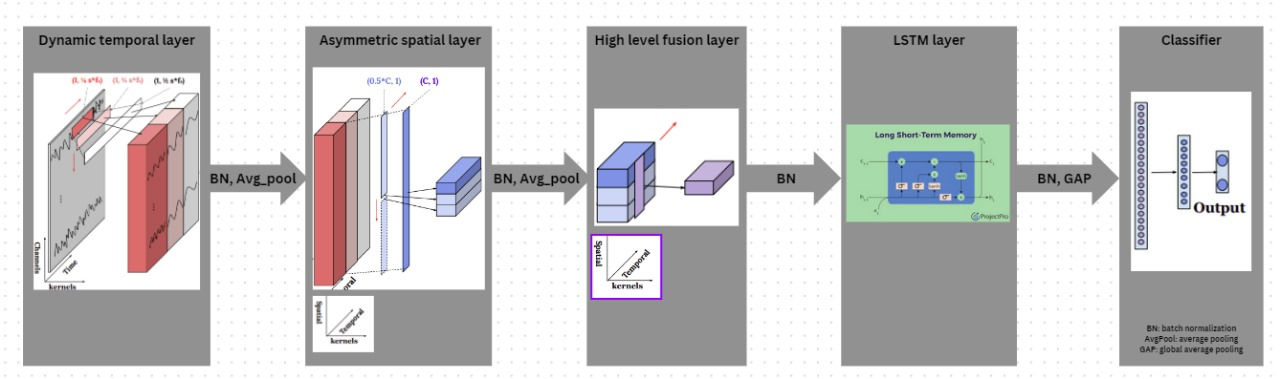
\includegraphics[width=\textwidth]{diagram.jpeg}
    \caption{New model architecture}
    \label{fig:yourlabel}
  \end{figure*}

\subsection*{Spatial Assymmetric Layer}
The assymmetric spatial layer is designed to capture the spatial patterns reflecting structural and functional assymetry of the human brain. It particularly focuses on differences between left and right hemispheres.It uses multi scale  $1$ D convolutional kernels to analyze the data. These patterns are aptly captured the spatial arrangement of the EEG channels on the scalp.
\subsubsection*{Types of Spatial Kernels}

\begin{itemize}
    \item \textbf{Global Kernel:} This kernel has a size of \((c, 1)\), where \(c\) is the total number of channels. It spans all channels at a time enabling it to capture global spatial information from the entire array of EEG channels.
    \item \textbf{Hemisphere Kernel:} This kernel, size \((0.5 \cdot c, 1)\) with a stride of \((0.5 \cdot c, 1)\), specifically targets the relationships between the left and right hemispheres. The kernel is shared between corresponding locations on each hemisphere, facilitating the extraction of asymmetrical patterns without overlapping.
\end{itemize}
After convolution with the global kernel, the output feature map is given by:
\begin{align*}
    \text{Output feature map} &\Rightarrow \dim(n, 1, f)
\end{align*}

After convolution with each hemisphere kernel:
\begin{align*}
    \text{1\textsuperscript{st} half: feature map} &\Rightarrow \dim(n, 1, f) \\
    \text{2\textsuperscript{nd} half: feature map} &\Rightarrow \dim(n, 1 , f)
\end{align*}

Concatenating the two halves yields:
\begin{align*}
    \text{Concatenated feature map} &\Rightarrow \dim(n, 3, f)
\end{align*}

Both the kernels apply $1$ D convolution operation to the output of the dynamic temporal layer. After convolution, feature maps are passed through the Leaky-Relu to introduce non linearity followed by average pooling and batch normalisation.

\subsection*{High Level Fusion Layer}
This layer integrates the spatial information extracted from the Assymmetric spatial layer from global and hemisphere kernels. It is is $1$ D convolutional layer with kernel size $(3, 1)$. Subsequently, Leaky-Relu,average pooling layer, batch normalisation and GAP layer are applied on the convolutional output.

This gives a high level representation of the data which is fed to the fully connected network fro training which can learn complex relationships between the fused features.To produce probability distribution over the target classes,a softmax fucntion is used.

\subsection*{LSTM Layer}
The input to the LSTM layer is the output of the fusion layer which is batch normalised. The mean is computed along the last dimension, preparing the data to have suitable shape to pass through LSTM.The LSTM structure is defined with a specified number of input features \((\text{num\_S})\), a hidden state size \((\text{lstm\_hidden})\), and it is set to have the batch data first \((\text{batch\_first} = \text{True})\). This configuration is crucial as it dictates how the LSTM processes the input data and the dimensionality of the output.
The LSTM processes the input sequence in a recurrent fashion, updating its hidden states and cell states at each time step.
It provides two outputs the hidden states for all time steps and the cell states. For our classification the last hidden state is used for the final classification.
The \texttt{fc\_lstm} is a sequence of fully connected layers (linear layers in PyTorch) with a ReLU activation and dropout for regularization. The final layer maps the hidden state to the number of classes for classification.

% \begin{figure}[h]
%     \centering
%     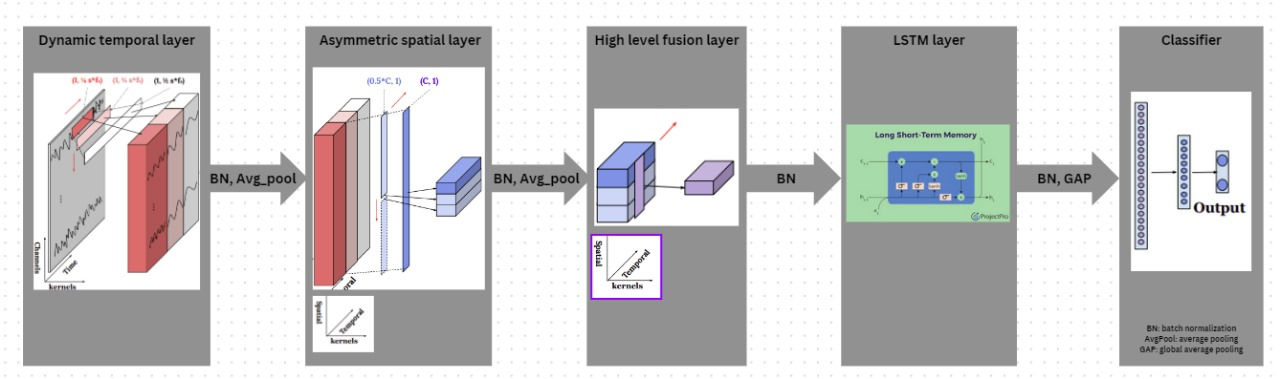
\includegraphics[width=0.5\textwidth]{diagram.jpeg} % Adjust the path and the scaling factor
%     \caption{New model architecture} % Caption for the image
%     \label{New model architecture} % Label for referencing the image elsewhere in the text
% \end{figure}

  

\section{Implementation and Results}
The proposed Tsception model was trained on data of 15 subjects. The 10-fold cross-validation method was carried out on the data. One fold was used for testing, and the remaining 9 folds were used for training. The model was trained for 100 epochs with a batch size of 64. The model was trained using the Adam optimizer with a learning rate of $0.0001$ and a weight decay of $0.0001$. The ratio $\alpha$ used for the kernel window size was $0.125$, $0.25$, $0.5$. The number of hidden nodes in LSTM was kept as 128. The model was evaluated for two dimensions, Arousal' and Valence'. The model was evaluated using two important metrics: validation accuracy and F1 score.
The following training loss and validation loss vs epochs plots were obtained for the first 8 subjects without LSTM for a randomly picked trial.
\begin{figure}[h]
    \centering
    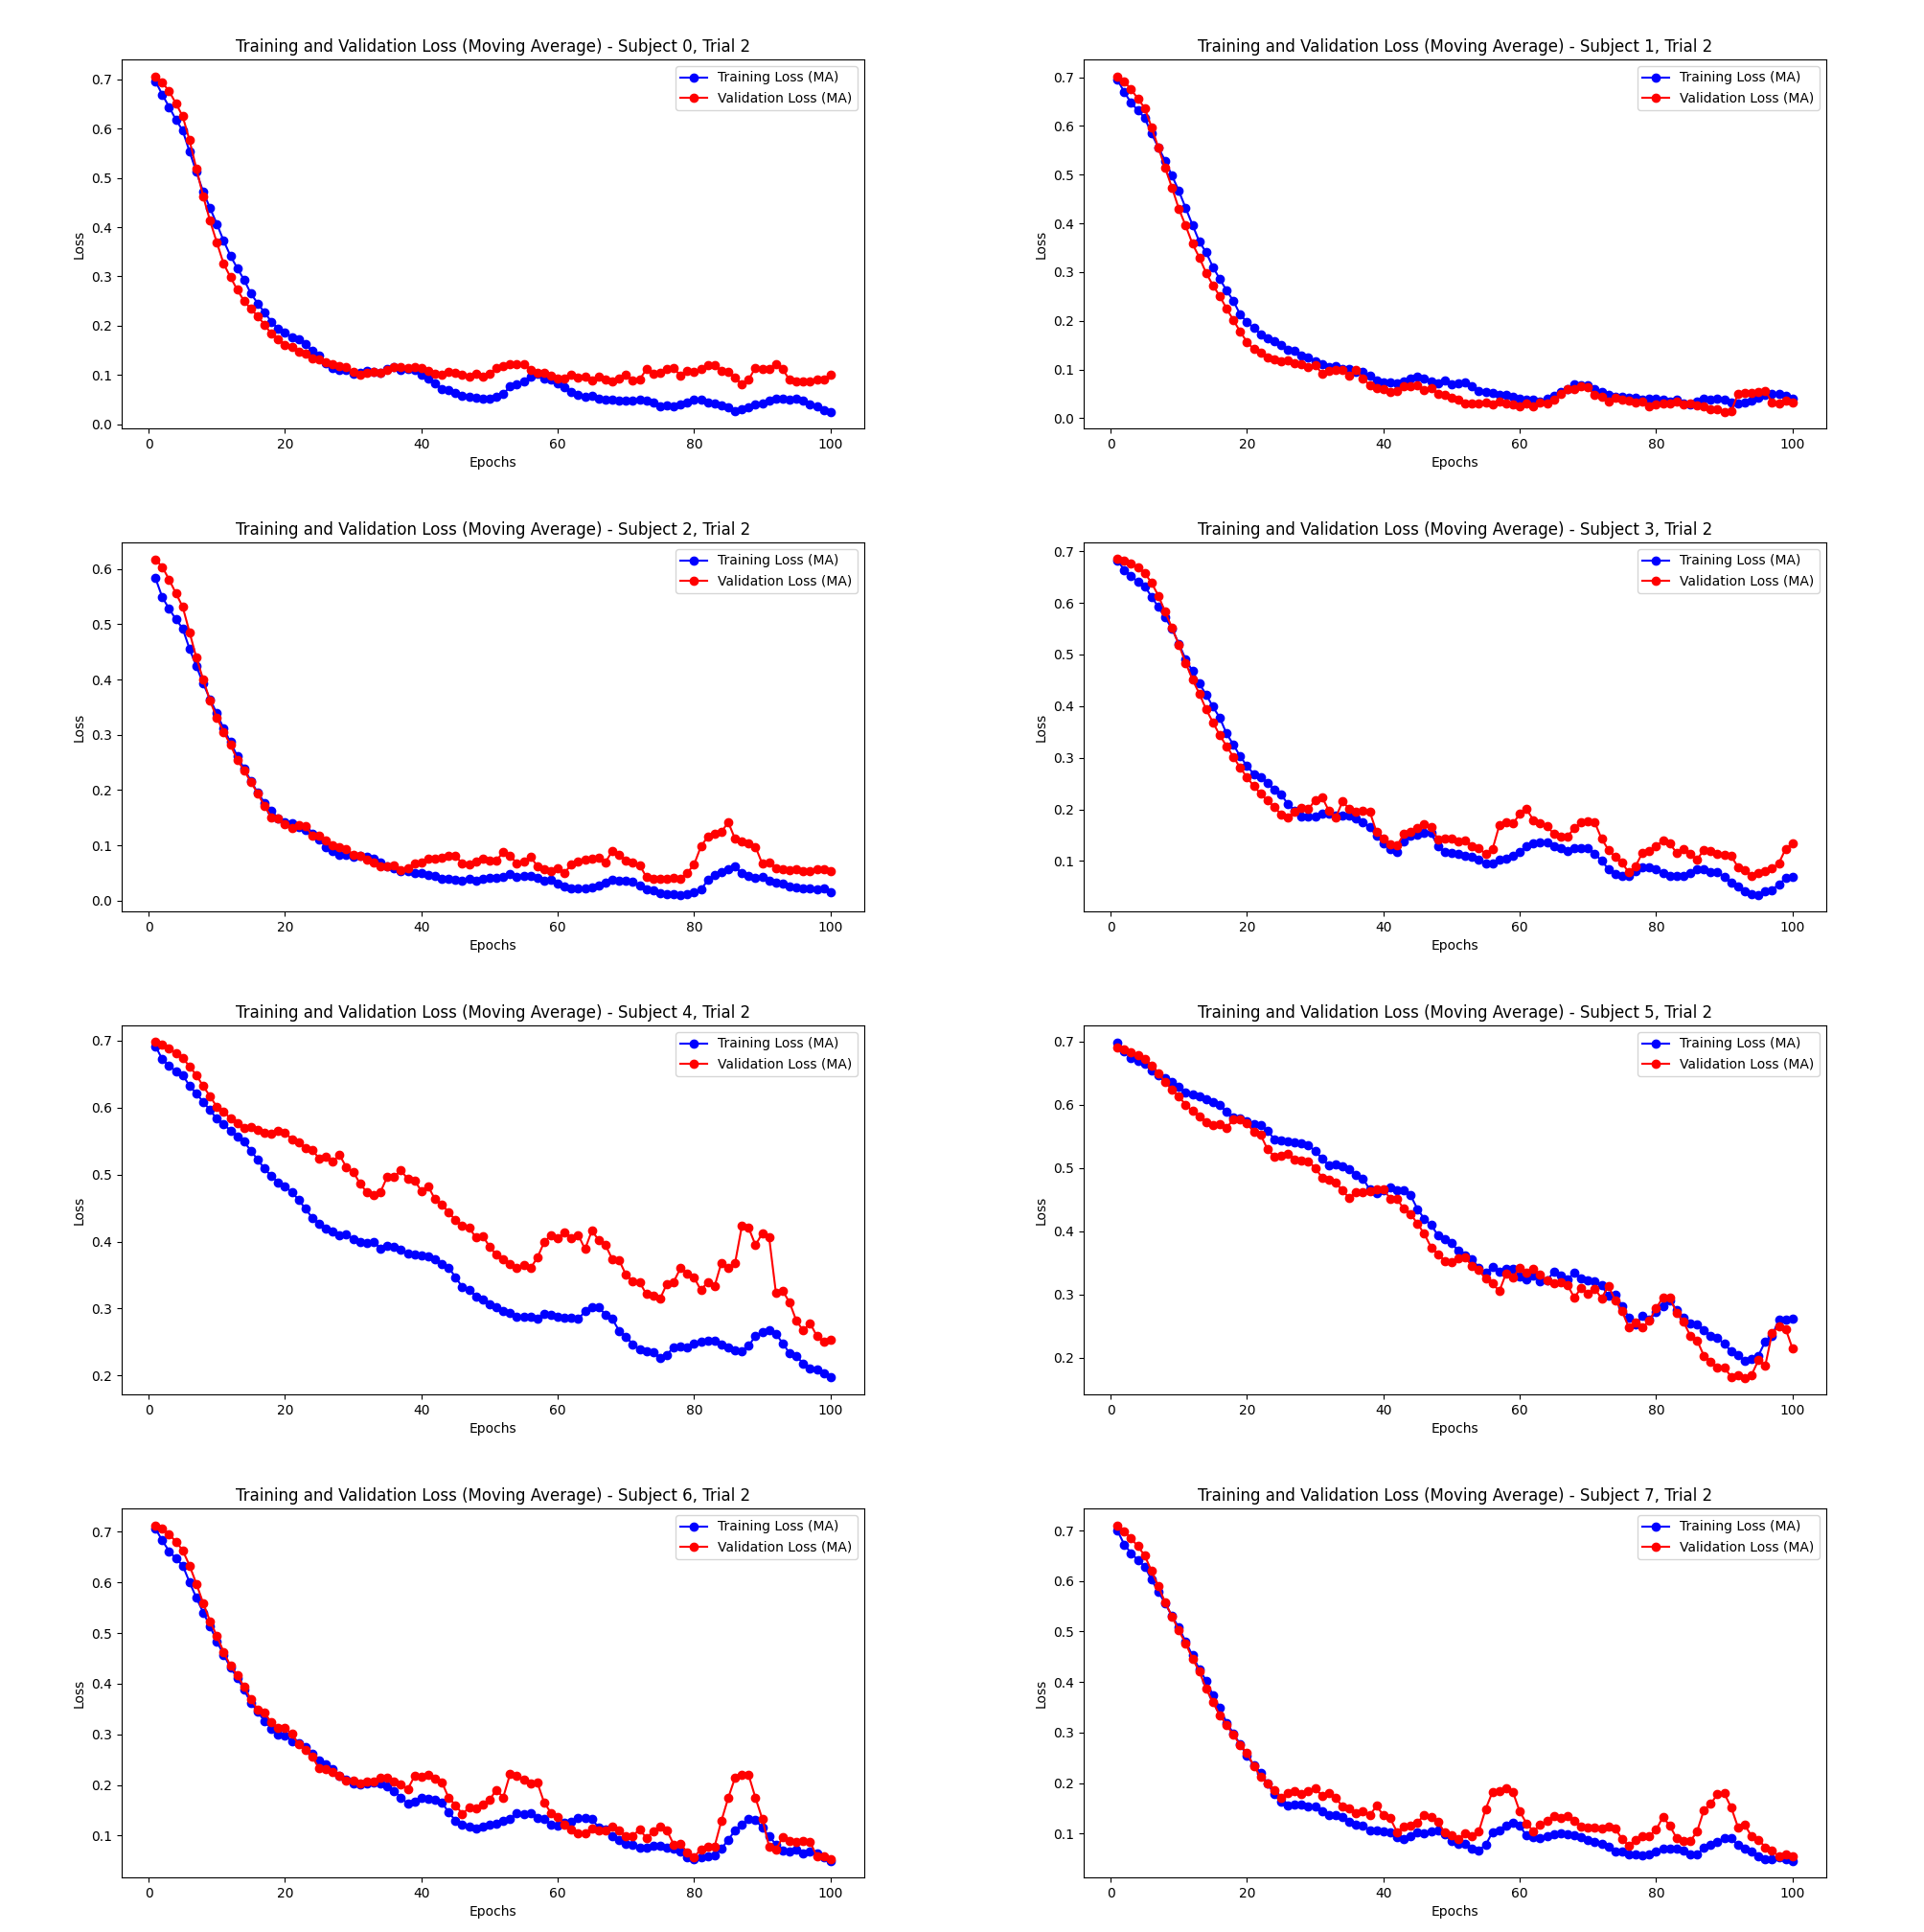
\includegraphics[width=0.5\textwidth, height = 10cm]{combined.png} % Adjust the path and the scaling factor
    \caption{Loss vs epochs without LSTM} % Caption for the image
    \label{loss vs epoch without LSTM} % Label for referencing the image elsewhere in the text
\end{figure}

The following training loss and validation loss vs epochs plots were obtained for the first 8 subjects without LSTM for a randomly picked trial.

\begin{figure}[h]
    \centering
    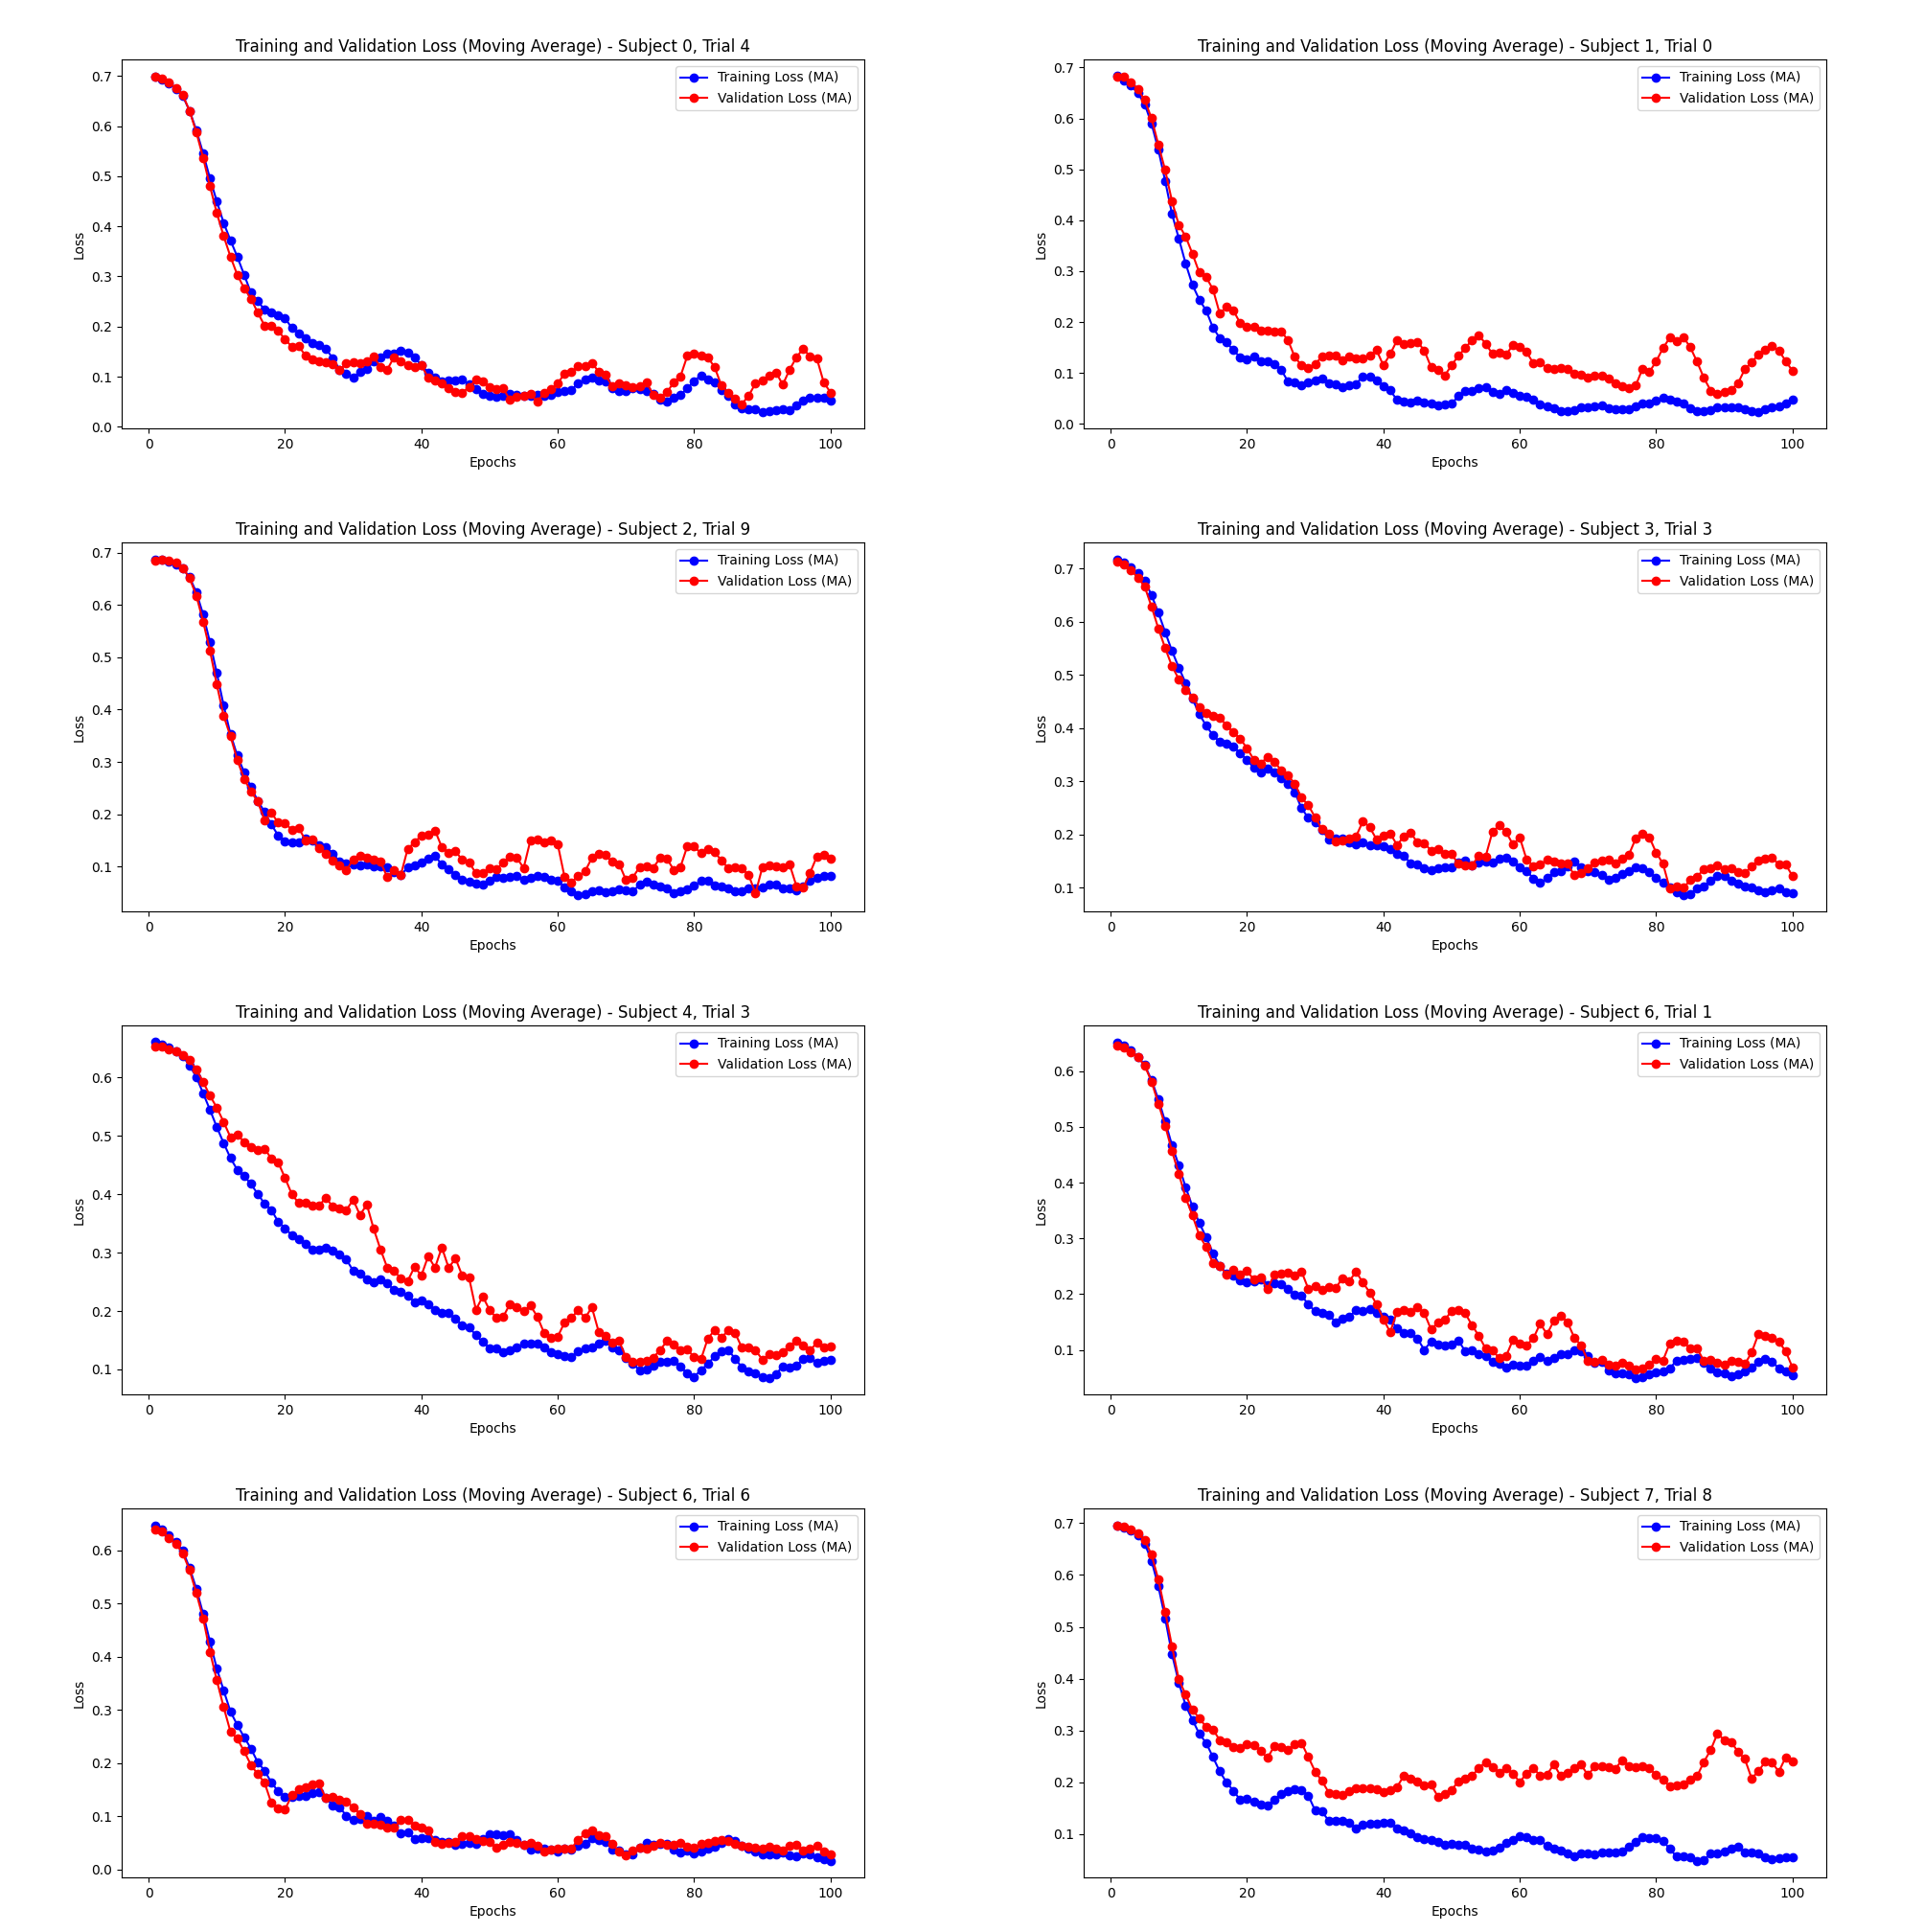
\includegraphics[width=0.5\textwidth, height =10cm]{new_combined.png} % Adjust the path and the scaling factor
    \caption{Loss vs epochs with LSTM} % Caption for the image
    \label{loss vs epoch with LSTM} % Label for referencing the image elsewhere in the text
\end{figure}

With LSTM, the loss decreases more steeply in the initial epochs compared to those without LSTMS. LSTMS contribute to faster convergence. Fluctuautions in the validation loss are lesser with using LSTM showing more robustness and generalizability of the model. Also the final loss values at the end of 100 epochs is lower for the Tsception model with LSTM than without.

The proposed model have an accuracy and F1 score higher than the original model for both the dimensions arousal and valence. The accuracy for arousal and valence show improvemnet with LSTM with accuracies of $0.9325$ and $0.926$ respectively as compared to older Tsception model with accuracies of $0.9162$ and $0.9156$ for arousal and valence dimensions respectively. ALong with this the F1 scores also show a significant improvement with scores of $0.944$ and $0.938$ with LSTM as compared to $0.923$ and $0.9185$ for older model.

The proposed model shows an overall improvement of $1.77$\% and $0.5$\% in accuracy for arousal and valence respectively. The F1 score also shows an improvement of $2.2$\% and $1.9$\% for arousal and valence dimensions respectively.
\begin{table}[ht]
    \centering
    \begin{tabular}{lcr} % alignment for each column (left, center, right)
    \toprule
    metric & with LSTM & Without LSTM  \\
    \midrule
    Arousal & 0.9325 & 0.9162 \\
    Valence & 0.9205 & 0.9156 \\
    \bottomrule
    \end{tabular}
    \caption{Accuracy comparison}
    \label{tab:example}
\end{table}
\begin{table}[ht]
    \centering
    \begin{tabular}{lcr} % alignment for each column (left, center, right)
    \toprule
    metric & with LSTM & Without LSTM  \\
    \midrule
    Arousal & 0.944 & 0.923 \\
    Valence & 0.938 & 0.9185 \\
    \bottomrule
    \end{tabular}
    \caption{F1 scores comparison}
    \label{tab:example}
\end{table}
    
    



\section{Conclusion}
This study presented an extended version of the TSception model, incorporating an LSTM layer to enhance the capability of capturing complex sequential temporal dynamics and spatial asymmetries from EEG data. The extended model, TSception-2, was rigorously evaluated against the original TSception model using the DEAP dataset for emotion analysis. The results were promising, showing that the inclusion of LSTM led to a notable improvement in both accuracy and F1 scores for the dimensions of arousal and valence.

The convergence analysis indicated that LSTM contributes to a faster and more robust learning process, as evidenced by steeper declines in loss during the initial training epochs and lesser fluctuations in validation loss, suggesting improved generalizability. The TSception-2 model achieved an accuracy improvement of 1.77\% for arousal and 0.5\% for valence, while F1 scores saw an enhancement of 2.2\% for arousal and 1.9\% for valence compared to the original TSception model.

These findings underscore the efficacy of LSTM layers in handling EEG signal variability and the non-stationary nature of emotional states. The comprehensive evaluation and interpretability analysis shed light on the network's functionality and highlighted the potential of deep learning methods in advancing BCI technologies for emotion recognition. Future work could explore the integration of other modalities and the application of the model in real-time systems, paving the way for innovative solutions in healthcare, gaming, and assistive technologies.


{
    \small
    \nocite{*}
    % \bibliographystyle{ieeenat_fullname}
    % \bibliography{main}
    
}

% WARNING: do not forget to delete the supplementary pages from your submission 
% \input{sec/X_suppl}
% \section{bibliography}
\begin{thebibliography}{9}
\bibitem{TSception2022}
\textit{TSception: Capturing Temporal Dynamics and Spatial Asymmetry from EEG for Emotion Recognition}.
ResearchGate, 2022.
\url{https://www.researchgate.net/publication/360127722_TSception_Capturing_Temporal_Dynamics_and_Spatial_Asymmetry_from_EEG_for_Emotion_Recognition}.
\end{thebibliography}

\end{document}